\documentclass[tikz,border=3pt]{standalone}
\usepackage[utf8]{inputenc}
\usepackage[T1]{fontenc}
\usepackage{lmodern}
\renewcommand{\familydefault}{\sfdefault}
\usepackage{sansmath}\sansmath
\usepackage[american]{circuitikz}
\usepackage{pgfplots}\pgfplotsset{compat=1.18,/pgf/number format/use comma,/pgf/number format/1000 sep={.}}
\usetikzlibrary{arrows.meta,calc,positioning,decorations.pathmorphing,patterns}
% paleta del sitio
\definecolor{nar}{HTML}{E8680C}\definecolor{narc}{HTML}{FFB35C}\definecolor{hielo}{HTML}{FFF3E8}
\definecolor{tinta}{HTML}{1D1D1F}\definecolor{gris}{HTML}{6E6E73}\definecolor{lila}{HTML}{7C5CF0}
\definecolor{azul}{HTML}{2F6FD6}\definecolor{menta}{HTML}{17A673}\definecolor{coral}{HTML}{E8342A}
\begin{document}
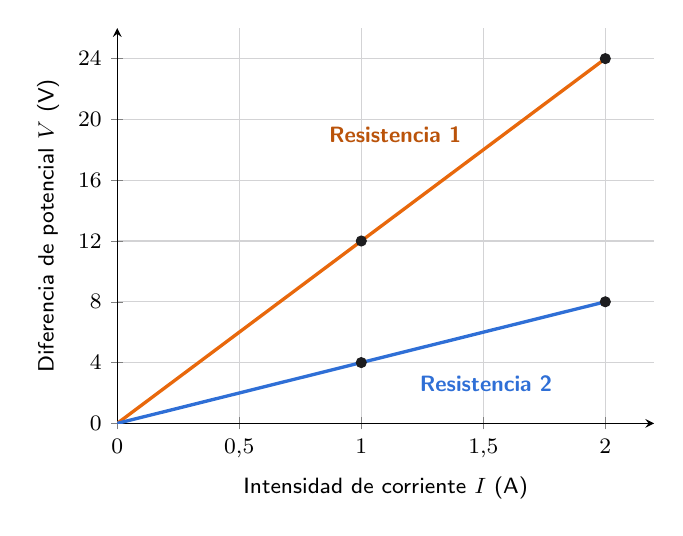
\begin{tikzpicture}[font=\small]
\begin{axis}[width=8.4cm,height=6.6cm,xmin=0,xmax=2.2,ymin=0,ymax=26,xtick={0,0.5,...,2},ytick={0,4,...,24},grid=major,grid style={gris!30},
  axis lines=left,xlabel={Intensidad de corriente $I$ (A)},ylabel={Diferencia de potencial $V$ (V)},tick label style={font=\footnotesize},label style={font=\footnotesize}]
\addplot[nar,very thick,domain=0:2] {12*x};
\addplot[azul,very thick,domain=0:2] {4*x};
\addplot[only marks,mark=*,mark size=1.8pt,tinta] coordinates {(1,12) (2,24) (1,4) (2,8)};
\node[font=\footnotesize\bfseries,text=nar!80!black,anchor=east] at (axis cs:1.45,19) {Resistencia 1};
\node[font=\footnotesize\bfseries,text=azul,anchor=west] at (axis cs:1.2,2.6) {Resistencia 2};
\end{axis}
\end{tikzpicture}
\end{document}
